\subsection{Room}
\label{cha:room}

In comparison of using Shared Preferences instead of Room it is possible to persist non-trivial amounts of structured data. The Room persistence library provides an abstraction layer over the SQLite database. It allows easier access to the database, but uses SQLite in the background.
The most important benefits are \cite{android_room}:

\begin{itemize}
    \item compile-time validation of SQL queries
    \item minimizes boilerplate code with annotations
    \item enables migrations \\
\end{itemize}

\noindent
The major components of Android Room are \cite{android_room}:

\begin{itemize}
    \item Database Class: main access point for the database connection
    \item Data Entities: tables of database
    \item Data Access Objects (DAOs): methods for querying, updating and deleting data in the database \\
\end{itemize}

In \cite{Figure_2} it is shown how theses components work together. The Room Database get the queries from the DAO and executes them. The result will then be stored in the entities via the getter/setter methods.

\begin{figure}[ht]
    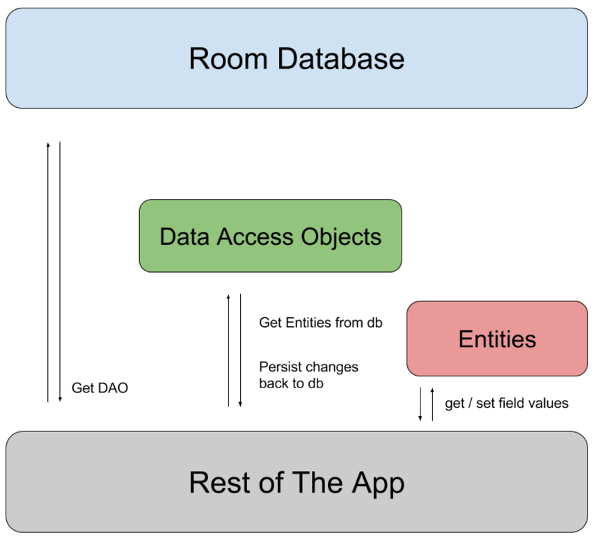
\includegraphics[width=\linewidth]{images/room_architecture.png}
    \caption{Architecture of Room \cite{Figure_2}}
    \label{fig:room_architecture}
\end{figure}

Example of a DAO for some table supporting a select, insert and delete statement:

\begin{lstlisting}[language=Kotlin]
@Dao
interface SomeTableDao {
    /**
     * @return all entries
     */
    @Query("SELECT * FROM some_table")
    fun getAll(): Flow<List<SomeEntry>>

    /**
     * insert a range of entries
     */
    @Insert(onConflict = 
        OnConflictStrategy.REPLACE
    )
    fun insertAll(vararg entries: SomeEntry)

    /**
     * delete all entries
     */
    @Query("DELETE FROM some_entry")
    fun deleteAll()
}
\end{lstlisting}